\chapter{Capa ETL con Apache Hop}
\label{chap:desarrollo_etl}

\lettrine{E}{l} éxito de un sistema de Business Intelligence radica en la calidad, consistencia y fiabilidad de sus datos. En esta fase central del proyecto se ha utilizado \textbf{Apache Hop}, una plataforma moderna e innovadora de orquestación y procesamiento de datos basada en metadatos, para diseñar e implementar los procesos de Extracción, Transformación y Carga (ETL).

Este capítulo detalla la arquitectura de los flujos de datos (\textit{Pipelines}) y de trabajo (\textit{Workflows}), exponiendo las decisiones técnicas tomadas para poblar el Datamart y calcular algorítmicamente los índices de riesgo de abandono escolar.

\section{Configuración del Entorno y Conexiones}

El ecosistema de Apache Hop se ha desplegado utilizando su imagen oficial de Docker (\textit{apache/hop-web}), garantizando un entorno de ejecución inmutable. La parametrización de las conexiones a bases de datos se ha resuelto de forma dinámica utilizando variables de entorno de la JVM pasadas en el momento de arranque del contenedor (e.g., \textit{-DDB\_SOURCE\_HOST}).

En la interfaz de Hop, se han configurado dos conexiones relacionales mediante el driver JDBC de PostgreSQL (ver Figura \ref{fig:hop_connections}):
\begin{itemize}
    \item \textbf{\textit{conn\_source}:} Conexión de solo lectura apuntando a la base de datos transaccional simulada.
    \item \textbf{\textit{conn\_dwh}:} Conexión de lectura y escritura apuntando al esquema dimensional del Data Warehouse.
\end{itemize}

\begin{figure}[htbp]
    \centering
    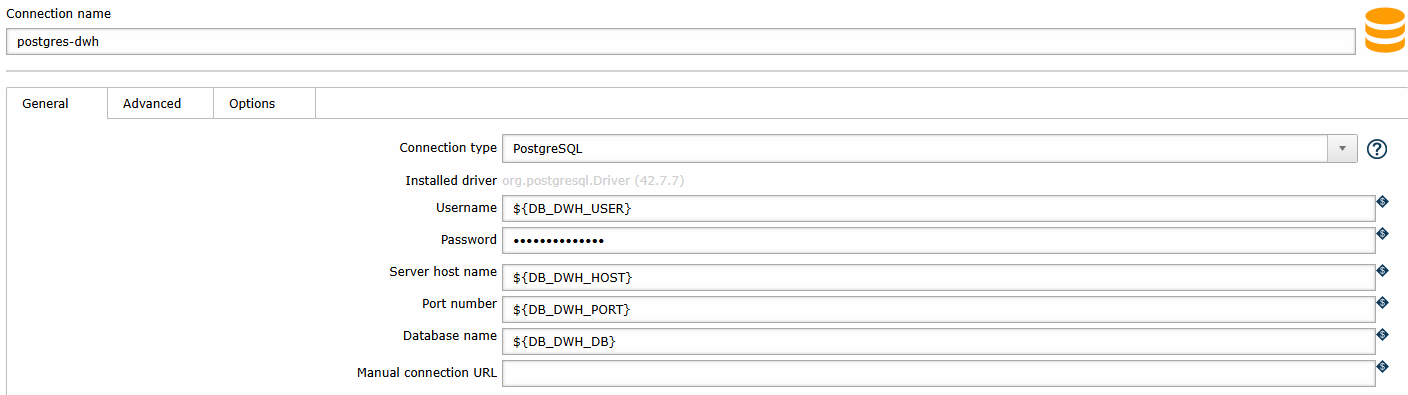
\includegraphics[width=0.9\textwidth]{imaxes/postgres-dwh_hop_conn.png}
    \caption{Configuración de la conexión \textit{postgres-dwh}.}
    \label{fig:hop_connections}
\end{figure}

\section{Análisis de Pipelines}

A continuación, se detalla el ciclo de vida del dato desglosando el funcionamiento técnico de cada uno de los pipelines (\textit{.hpl}) que componen el sistema ETL. Un pipeline en Apache Hop es un grafo dirigido acíclico (DAG) donde los nodos (\textit{Transforms}) ejecutan operaciones específicas (lectura, filtrado, cálculos) y las aristas (\textit{Hops}) canalizan el flujo de registros directamente en memoria.

\subsection{Volcado a Staging}

Para no sobrecargar la base de datos origen transaccional durante los cruces analíticos posteriores, el primer paso estricto de la arquitectura ETL consiste en realizar una clonación exacta de las tablas de producción hacia el esquema intermedio transitorio \textit{raw} (Staging Area). 

Como se aprecia en la Figura \ref{fig:extract_all_to_staging}, el pipeline \textit{extract\_all\_to\_staging.hpl} establece 14 hilos independientes de tipo \textit{Table Input} (origen) conectados a \textit{Table Output} (destino). Configurado como una extracción de tipo "volcado completo" (\textit{Full Load}), este flujo ejecuta un comando interno de truncado (\textit{Truncate=Y}) que vacía previamente las tablas de \textit{raw} para volcar los datos frescos del día en bloque. 

Una decisión de diseño fundamental documentada en este paso es la \textbf{ausencia de claves foráneas} en el esquema destino. Al no existir restricciones referenciales en la capa \textit{raw}, Hop puede paralelizar la inserción masiva de todas las entidades simultáneamente sin generar bloqueos lógicos por dependencias, minimizando drásticamente la ventana de tiempo de extracción.

\begin{figure}[htbp]
    \centering
    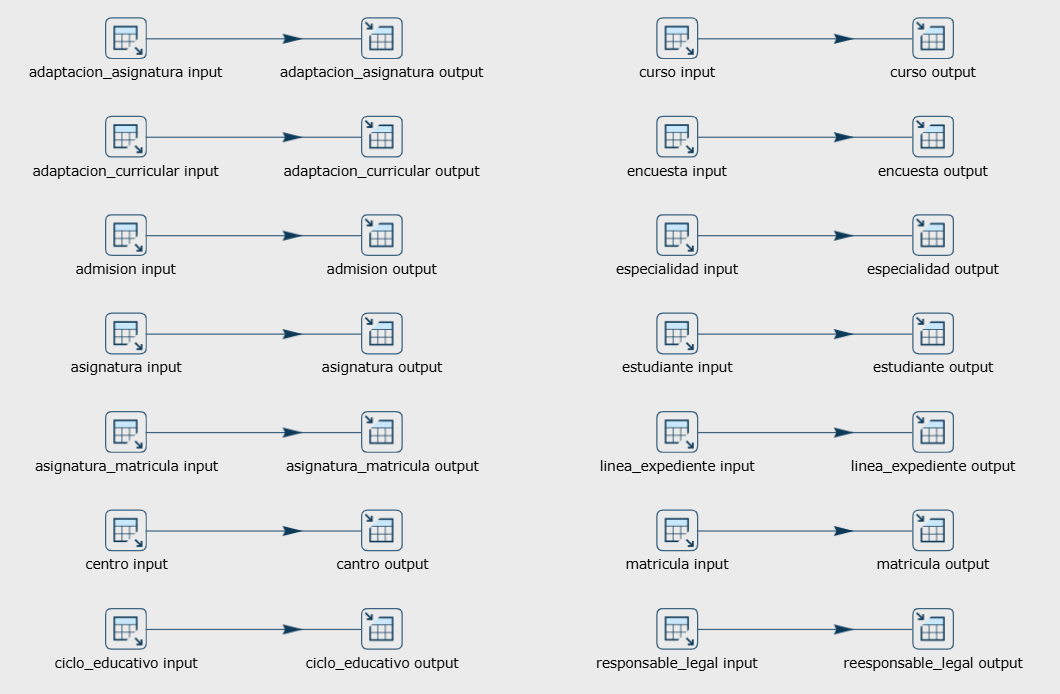
\includegraphics[width=1\textwidth]{imaxes/extract_all_to_staging.png}
    \caption{Flujo del pipeline \textit{extract\_all\_to\_staging.hpl}.}
    \label{fig:extract_all_to_staging}
\end{figure}

\subsection{Dimensión de Demograía Familiar}

El núcleo de las reglas de negocio del proyecto reside en este pipeline. Su misión es ingerir los datos brutos de la tabla de encuestas (\textit{raw.encuesta}) y destilarlos para construir una dimensión de baja cardinalidad que consolide los perfiles de riesgo socioeconómico. Su implementación técnica encadena operaciones aritméticas, lógicas condicionales y deduplicación (ver Figura \ref{fig:dim_demografia_familiar}):

\begin{enumerate}
    \item \textbf{Cálculo de Hijos a Cargo (\textit{Formula}):} Dado que la tabla origen \textit{raw.encuesta} solo informa del número total de integrantes del hogar, el pipeline calcula el número de hijos restando los adultos. Asume 1 adulto si no hay datos del segundo tutor, o 2 si los hay, garantizando matemáticamente un mínimo de 1 hijo.
    \item \textbf{Cálculos de Ratio y Consumo (\textit{Calculator}):} Se inicializan variables continuas dividiendo algebraicamente los ingresos brutos entre las unidades de consumo del hogar, obteniendo la \textit{renta\_unidades\_consumo}. Paralelamente, se divide \textit{num\_ordenadores} entre \textit{num\_hijos} calculados en el paso anterior para obtener la \textit{ratio\_ordenadores}.
    \item \textbf{Discretización de Variables Continuas (\textit{NumberRange}):} Las variables calculadas se segmentan en bandas analíticas fijas:
    \begin{itemize}
        \item \textit{nivel\_renta}: "Muy baja" ($<$ 7.000 €), "Baja" (7.000 € - 11.000 €) o "Media/Alta" ($>$ 11.000 €).
        \item \textit{disponibilidad\_ordenadores}: "Ninguno" (0), "Menos de 1 por hijo" (0.001 a 0.999), o "1 o mas por hijo" ($\ge$ 1).
    \end{itemize}
    \item \textbf{Máximo Nivel de Estudios (\textit{ValueMapper} y \textit{Formula}):} El pipeline transforma los niveles de estudio de ambos progenitores en un peso numérico (Universitarios=3, Secundarios=2, Primarios=1, Sin Estudios=0), aplica una función MAX([peso\_estudios\_1], [peso\_estudios\_2]) para quedarse con el nivel más alto del hogar, y vuelve a traducir ese número a cadena de texto (\textit{max\_nivel\_estudios}).
    \item \textbf{Asignación de Puntos de Riesgo (\textit{ValueMapper}):} Se inyectan los pesos definidos por el negocio para calcular el riesgo de abandono:
    \begin{itemize}
        \item \textit{pts\_nivel\_renta}: Muy baja (15 pts), Baja (7 pts), Media/Alta (0 pts).
        \item \textit{pts\_nivel\_estudios}: Sin Estudios (10 pts), Primarios (6 pts), Secundarios (2 pts), Universitarios (0 pts).
        \item \textit{pts\_disponibilidad\_ordenadores}: Ninguno (5 pts), Menos de 1 (2 pts), 1 o más (0 pts).
        \item \textit{pts\_internet}: Sin acceso (3 pts), Con acceso (0 pts).
    \end{itemize}
    \item \textbf{Ecuación Maestra (\textit{Formula}):} Se materializa la variable predictiva final sumando todos los factores: [pts\_disponibilidad\_ordenadores] + [pts\_internet] + [pts\_nivel\_estudios] + [pts\_nivel\_renta].
    \item \textbf{Optimización de Cardinalidad (\textit{SortRows - unique\_rows=Y}):} Para evitar que la dimensión crezca con cada estudiante, un nodo ordena por los atributos cualitativos y descarta los duplicados exactos en memoria. De miles de encuestas, el Data Warehouse solo almacena las combinaciones únicas posibles.
    \item \textbf{Carga en Datamart (\textit{Combination lookup/update}):} Se vuelcan los perfiles deduplicados en \textit{dwh.dim\_demografia\_familiar}, generando una clave subrogada autoincremental (\textit{id\_demografia\_familiar}) que será utilizada posteriormente por la tabla de hechos.
\end{enumerate}

\begin{figure}[htbp]
    \centering
    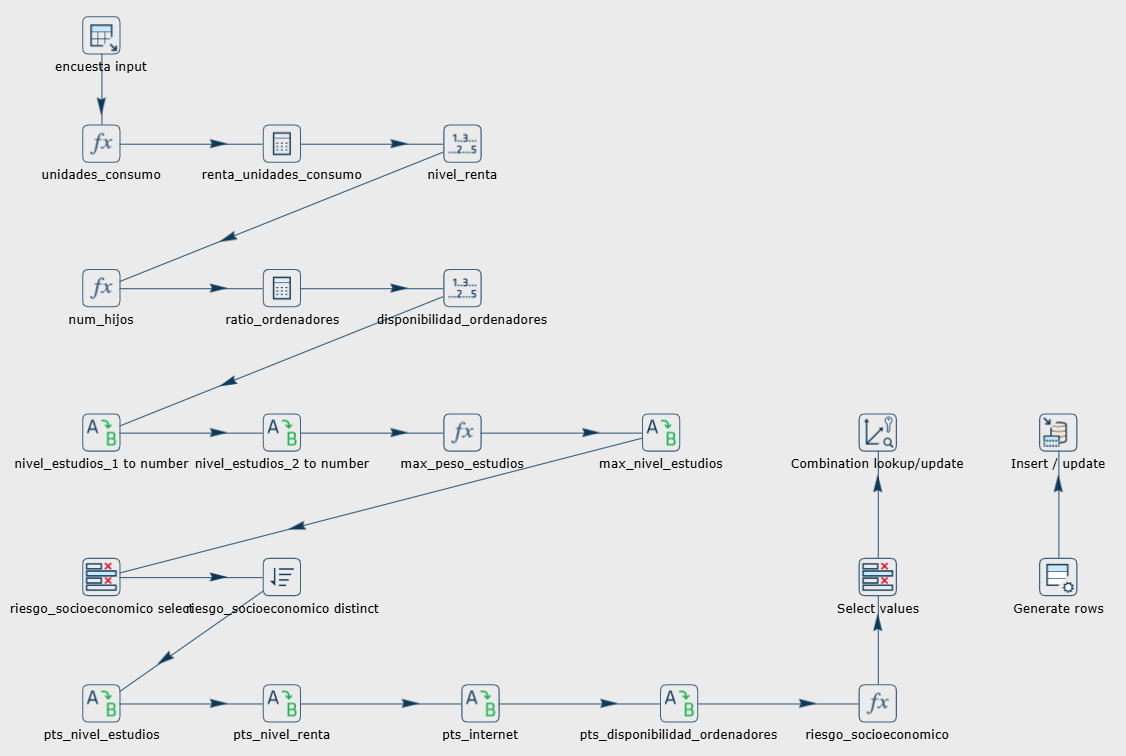
\includegraphics[width=1\textwidth]{imaxes/dim_demografia_familiar.png}
    \caption{Flujo del pipeline \textit{dim\_demografia\_familiar.hpl}.}
    \label{fig:dim_demografia_familiar}
\end{figure}

\subsection{Dimensión de Estudiante}

La dimensión del alumnado requiere un modelado avanzado, ya que la casuística de un estudiante no es estática: puede cambiar de domicilio, de tutor legal o de situación familiar a lo largo de los años. Si el sistema simplemente sobrescribiese estos datos, se perdería el contexto socioeconómico real que tenía el alumno cuando obtuvo una calificación pasada. Para solventarlo, este pipeline implementa un algoritmo SCD (Slowly Changing Dimension) Tipo 2 apoyado en la limpieza previa de cadenas (ver Figura \ref{fig:dim_estudiante}).

\begin{enumerate}
    \item \textbf{Cruce y Limpieza de Cadenas (\textit{MergeJoin} y \textit{FieldSplitter}):} El flujo extrae asíncronamente las entidades \textit{raw.estudiante} y \textit{raw.responsable\_legal}, ordenándolas en memoria (\textit{SortRows}) para ejecutar un \textit{Merge Join} tipo LEFT OUTER por el campo \textit{cod\_responsable}. A continuación, un nodo \textit{FieldSplitter} disecciona la cadena cruda de la dirección separándola por comas en las columnas \textit{calle\_portal}, \textit{puerta}, \textit{cp} y \textit{ciudad}.
    \item \textbf{Casteo de Datos (\textit{ReplaceString} y \textit{SelectValues}):} El nodo \textit{ReplaceString} elimina la subcadena "CP " de los códigos postales, permitiendo que el paso subsiguiente (\textit{SelectValues}) lo formatee analíticamente como un tipo numérico (Integer) y renombre simultáneamente las variables de los tutores a la nomenclatura final del DWH.
    \item \textbf{Algoritmo SCD Tipo 2 (\textit{Dimension lookup/update}):} El motor principal del pipeline es este nodo nativo de Hop, configurado para rastrear el ciclo de vida del \textit{num\_expediente} (Clave Natural) gestionando automáticamente una clave subrogada \textit{id\_estudiante} (autoincremental), un contador de \textit{version} y las marcas temporales \textit{date\_from} y \textit{date\_to}. La maestría de esta configuración reside en la micro-gestión de actualizaciones campo a campo:
    \begin{itemize}
        \item \textbf{\textit{Punch through} (Comportamiento SCD Tipo 1):} Campos intrínsecos como el \textit{dni}, \textit{nombre} o \textit{fecha\_nacimiento}. Una corrección en origen de estos datos no justifica crear un nuevo histórico; Hop sobrescribe el valor directamente en todas las versiones pasadas de ese estudiante.
        \item \textbf{\textit{Insert} (Comportamiento SCD Tipo 2):} Campos dependientes del contexto socioeconómico, como \textit{cod\_responsable}, \textit{calle\_portal}, \textit{ciudad} y \textit{monoparental}. Si Hop detecta una mutación en cualquiera de estos campos frente al registro vigente en el DWH, congela la fila antigua (estampando el \textit{date\_to} actual), e inserta una nueva fila virgen con la versión incrementada y un nuevo \textit{id\_estudiante}.
        \item \textbf{\textit{Update}:} Datos de contacto secundarios como el \textit{email}, que se actualizan silenciosamente en la versión activa sin generar ruido histórico.
    \end{itemize}
\end{enumerate}

\begin{figure}[htbp]
    \centering
    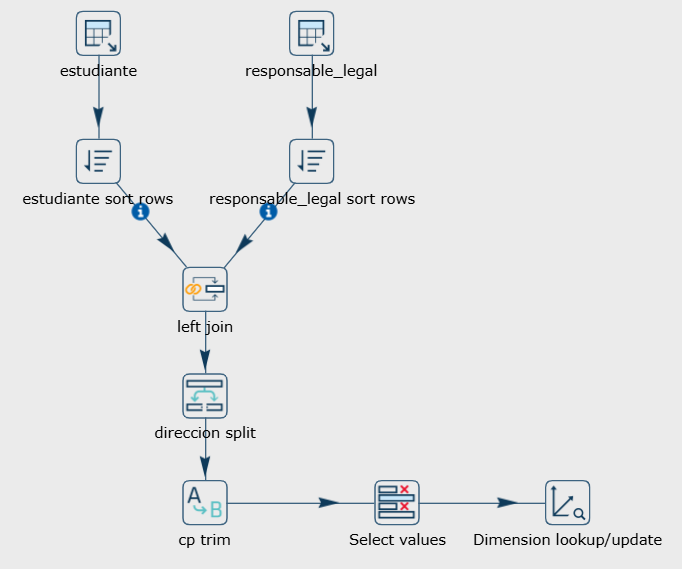
\includegraphics[width=1\textwidth]{imaxes/dim_estudiante.png}
    \caption{Flujo del pipeline \textit{dim\_estudiante.hpl}.}
    \label{fig:dim_estudiante}
\end{figure}

\subsection{Dimensión de Tiempo}

A diferencia de un calendario estándar por días o meses, este sistema requiere una dimensión de tiempo puramente académica que categorice los momentos evaluativos de un alumno (por ejemplo, "Curso 2023-2024, 1ª Evaluación"). Este pipeline infiere automáticamente estas temporalidades desde los propios registros transaccionales (ver Figura \ref{fig:dim_tiempo}).

\begin{enumerate}
    \item \textbf{Cruce Transaccional (\textit{MergeJoin}):} El flujo no lee de una tabla maestra explícita, sino que extrae las operaciones transaccionales \textit{raw.linea\_expediente} y \textit{raw.matricula}. Tras ordenar ambas por \textit{cod\_matricula} mediante nodos \textit{SortRows}, aplica un cruce de tipo INNER JOIN para asociar la \textit{evaluacion} en la que se puso cada nota con el \textit{curso\_academico} de la matrícula correspondiente.
    \item \textbf{Extracción del Dominio (\textit{SortRows - unique\_rows=Y}):} De los cientos de miles de líneas de expediente cruzadas, se extrae el dominio temporal real filtrando únicamente los pares únicos de \textit{curso\_academico} y \textit{evaluacion}, purificando así la dimensionalidad.
    \item \textbf{Análisis Léxico Condicional (\textit{FilterRows}):} Un paso crítico para el negocio es aislar si una evaluación es la definitiva o una parcial (fundamental para el pipeline posterior de \textit{fact\_rendimiento\_anual}). Un nodo \textit{FilterRows} analiza léxicamente el texto de la evaluación buscando la subcadena "Final" (evaluando múltiples casuísticas mediante condicionales \texttt{CONTAINS} encadenados con operadores \texttt{OR}: "Final", "final", "FINAL").
    \item \textbf{Bifurcación de Flujo Dirigido:} Dependiendo del resultado del filtro anterior, Hop enruta el dato físicamente por dos caminos paralelos. Si el filtro resulta verdadero, el registro se desvía a un nodo \textit{Add constants true} que inyecta la variable booleana (is\_final = Y). Si es falso, viaja por la rama inferior a \textit{Add constants false} (is\_final = N). Ambas ramas se reconcilian posteriormente en un nodo \textit{Dummy} integrador.
    \item \textbf{Carga Híbrida (\textit{Combination lookup} + \textit{Update}):} El pipeline implementa un patrón avanzado de persistencia en Hop. Primero, el nodo \textit{Combination lookup/update} consolida las claves (\textit{curso\_academico} y \textit{evaluacion}) e inserta la fila generando automáticamente la clave subrogada \textit{id\_tiempo}. Como este paso nativo no admite insertar atributos no-clave simultáneamente, el flujo encadena de forma síncrona un paso \textit{Update}. Este busca el \textit{id\_tiempo} recién instanciado y le hace un UPDATE para persistir el metadato booleano \textit{is\_final} en la base de datos de destino.
\end{enumerate}

\begin{figure}[htbp]
    \centering
    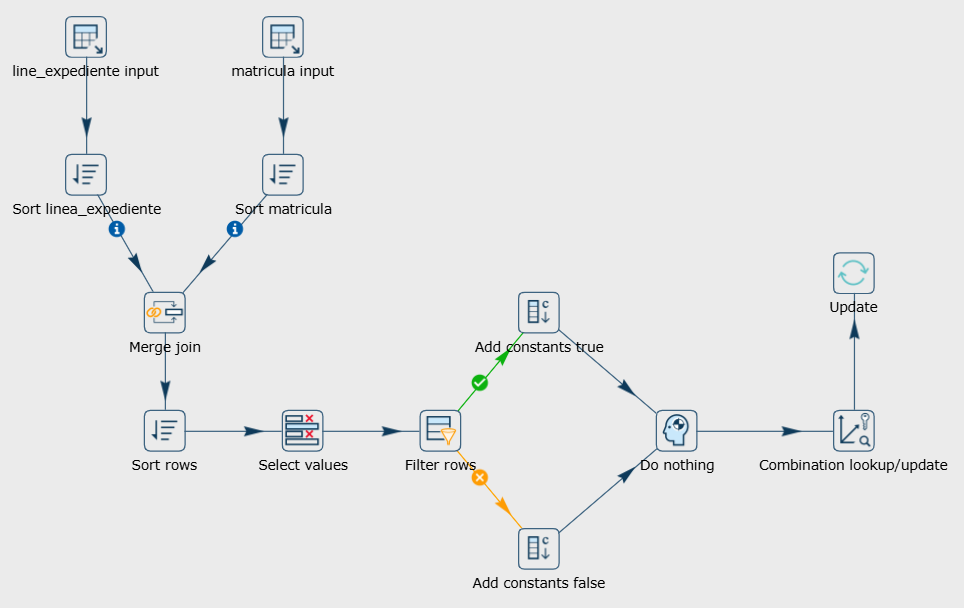
\includegraphics[width=1\textwidth]{imaxes/dim_tiempo.png}
    \caption{Flujo del pipeline \textit{dim\_tiempo.hpl}.}
    \label{fig:dim_tiempo}
\end{figure}

\subsection{Dimensión de Asignatura}

El modelo de asignaturas en el sistema origen transaccional presenta una arquitectura relacional altamente normalizada (en "Copo de Nieve"). Para modelarlo en el Data Warehouse bajo un esquema de Estrella óptimo para lectura, este pipeline colapsa jerarquías relacionales en una única fila dimensional (ver Figura \ref{fig:dim_asignatura}).

\begin{enumerate}
    \item \textbf{Ingesta y Búsquedas en Cascada (\textit{DBLookup}):} Hop extrae \textit{raw.asignatura} y, mediante tres nodos \textit{DBLookup} encadenados, recorre las claves foráneas hacia arriba. Primero recupera el \textit{num\_optativas} desde la tabla \textit{raw.curso}; después, obtiene la \textit{especialidad} y su ciclo asociado desde \textit{raw.especialidad}; y finalmente, extrae el marco normativo (\textit{real\_decreto}, \textit{decreto\_autonomico}) desde \textit{raw.ciclo\_educativo}.
    \item \textbf{Consolidación (\textit{SelectValues} y \textit{Combination lookup}):} Una vez que todas las ramas jerárquicas han sido aplanadas en un único vector, se purgan las claves intermedias y se genera el registro en la dimensión destino con su \textit{id\_asignatura} correspondiente.
\end{enumerate}

\begin{figure}[htbp]
    \centering
    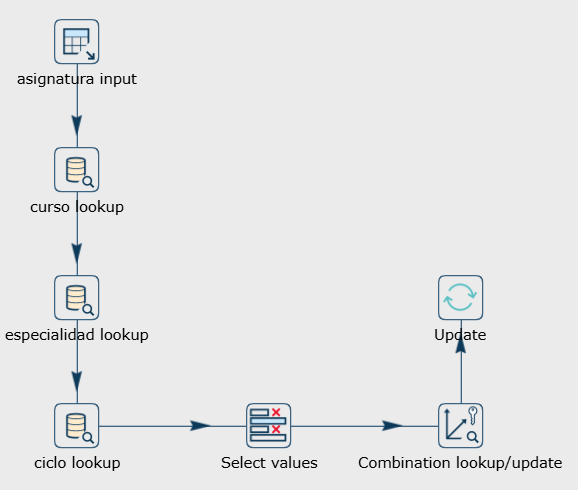
\includegraphics[width=1\textwidth]{imaxes/dim_asignatura.png}
    \caption{Flujo del pipeline \textit{dim\_asignatura.hpl}.}
    \label{fig:dim_asignatura}
\end{figure}

\subsection{Dimensión de Curso}

Esta dimensión no solo almacena los metadatos del curso y ciclo, sino que alberga una regla de negocio fundamental: determinar la edad teórica esperada para un alumno en cada nivel, lo cual permitirá posteriormente a la tabla de hechos calcular el desfase de edad (indicador clave de repetición y riesgo académico, ver Figura \ref{fig:dim_curso}).

\begin{enumerate}
    \item \textbf{Mapeo de Nivel Educativo (\textit{ValueMapper}):} Tras aplanar el curso, la especialidad y el ciclo educativo, un nodo inyecta paramétricamente la edad teórica de acceso al ciclo mediante pares clave-valor (ej. "PRI" $\rightarrow$ 5 años, "ESO" $\rightarrow$ 11 años, "BAC" $\rightarrow$ 15 años).
    \item \textbf{Cálculo Algebraico de Edad Ideal (\textit{Calculator}):} Un nodo matemático suma dinámicamente el número ordinal del curso a la edad base del ciclo. Así, un alumno en 3º de la ESO (ciclo base 11) tiene una \textit{edad\_ideal} de 14 años. Este valor precalculado se consolida permanentemente en \textit{dim\_curso}.
\end{enumerate}

\begin{figure}[htbp]
    \centering
    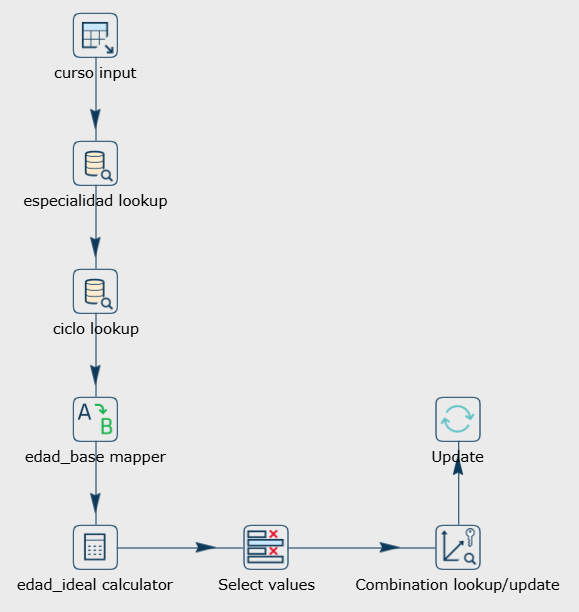
\includegraphics[width=1\textwidth]{imaxes/dim_curso.png}
    \caption{Flujo del pipeline \textit{dim\_curso.hpl}.}
    \label{fig:dim_curso}
\end{figure}

\subsection{Dimensión de Adaptación}

El registro transaccional de adaptaciones curriculares en los centros suele ser un campo de texto libre con la patología o motivo de la adaptación, dificultando su explotación analítica. Este pipeline actúa como un motor de extracción de reglas clínicas (ver Figura \ref{fig:dim_adaptacion}).

\begin{enumerate}
    \item \textbf{Limpieza de Dominio (\textit{SortRows} y \textit{RowGenerator}):} Dado que la mayoría del alumnado no presenta adaptaciones, el flujo genera sintéticamente una fila "Ninguna" para asegurar la integridad referencial en el modelo de estrella, y posteriormente extrae la lista de tipos únicos registrados en el histórico.
    \item \textbf{Clasificación Clínica por Expresiones Regulares (\textit{RegexEval}):} Dos nodos paralelos aplican potentes patrones Regex sobre el texto crudo:
    \begin{itemize}
        \item \textbf{\textit{is\_discapacidad}:} Busca que contenga (TND, Discalculia, Dislexia, Motórica, Visual, Asma, Mutismo, TDAH, TEA) para identificar discapacidades fisiológicas o neuropsicológicas.
        \item \textbf{\textit{is\_compensatoria}:} Rastrea que inclya (Absentismo, Ludopatía, Acogimiento, Convivencia, Ciberacoso, Conducta, Intercultural, Social, Inestabilidad, Inmersión, Lingüística) para aislar intervenciones estrictamente sociológicas.
    \end{itemize}
    \item \textbf{Ponderación de Severidad (\textit{ValueMapper} y \textit{Calculator}):} Cada tipología desencadena un peso distinto (10 puntos para las fisiológicas, 5 puntos para las sociológicas). Un nodo matemático suma los puntos creando la métrica unificada \textit{riesgo\_adaptacion}.
\end{enumerate}

\begin{figure}[htbp]
    \centering
    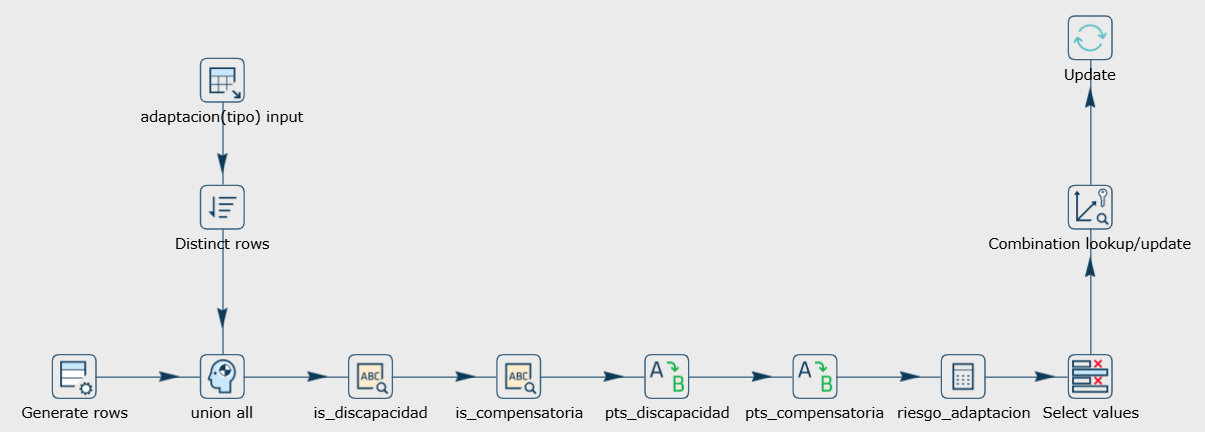
\includegraphics[width=1\textwidth]{imaxes/dim_adaptacion.png}
    \caption{Flujo del pipeline \textit{dim\_adaptacion.hpl}.}
    \label{fig:dim_adaptacion}
\end{figure}

\subsection{Dimensión de Centro}

El pipeline del centro educativo, aunque estructuralmente sencillo al procesar un catálogo estático y reducido de registros, encapsula lógicas de limpieza para la geolocalización analítica. El campo crudo \textit{direccion} se somete a un nodo \textit{FieldSplitter} que particiona los componentes por su coma delimitadora (en las columnas Calle, CP, y Ciudad), se limpia iterativamente la cadena del código postal eliminando el prefijo literario "CP " (\textit{ReplaceString}), y se fuerza su formateo en base de datos al tipo nativo Integer en un paso \textit{SelectValues} previo a la generación de la clave autoincremental \textit{id\_centro} (ver Figura \ref{fig:dim_centro}).

\begin{figure}[htbp]
    \centering
    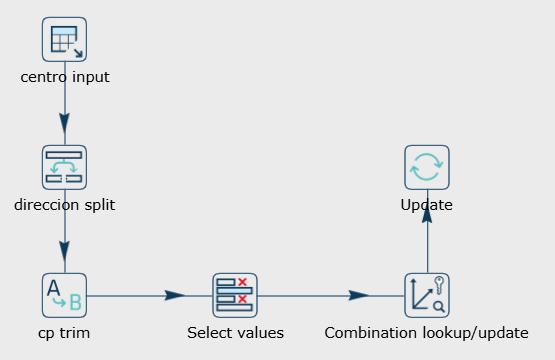
\includegraphics[width=1\textwidth]{imaxes/dim_centro.png}
    \caption{Flujo del pipeline \textit{dim\_centro.hpl}.}
    \label{fig:dim_centro}
\end{figure}

\subsection{Tabla de Hechos de Calificaciones}

Este es el pipeline central del sistema. Su objetivo es poblar la tabla de hechos atómica \textit{fact\_calificaciones}, cruzando los eventos transaccionales con todas las dimensiones construidas previamente y calculando métricas volátiles en el momento del evento (ver Figuras \ref{fig:fact_calificaciones_p1} y \ref{fig:fact_calificaciones_p2}).

\begin{enumerate}
    \item \textbf{Ingesta y Cruce Base (\textit{Table Input}, \textit{SortRows}, \textit{DBLookup}):} El flujo arranca extrayendo las calificaciones desde \textit{raw.linea\_expediente}, ordenándolas en memoria, y utilizando un nodo \textit{DBLookup} ("\textit{matricula lookup}") contra \textit{raw.matricula} para heredar metadatos vitales como la \textit{fecha} formal de matriculación, el \textit{curso\_academico} y el \textit{cod\_centro}.
    \item \textbf{Resolución de Claves Estáticas (\textit{DBLookup} en Cascada):} A continuación, se encadenan cuatro nodos idénticos de tipo \textit{DBLookup} que interrogan a las dimensiones estáticas (\textit{dim\_asignatura}, \textit{dim\_centro}, \textit{dim\_curso} y \textit{dim\_tiempo}) cotejando las claves naturales para extraer sus identificadores subrogados (\textit{id\_asignatura}, etc.). Críticamente, del nodo "\textit{dim\_curso lookup}" no solo se extrae la clave, sino que se arrastra la variable precalculada \textit{edad\_ideal}.
    \item \textbf{Gestión de Nulos en Adaptaciones (\textit{StreamLookup} e \textit{IfNull}):} Para resolver la dimensión de adaptaciones curriculares, el flujo lee asíncronamente las tablas \textit{raw} de adaptaciones, hace un \textit{StreamLookup} en memoria, e implementa un nodo \textit{IfNull} programado para inyectar la cadena "Ninguna" si el alumno no presenta patologías registradas. Un \textit{DBLookup} posterior extrae su \textit{id\_adaptacion}.
    \item \textbf{Resolución Temporal SCD2 (\textit{Dimension Lookup}):} Para enlazar la dimensión del estudiante, se emplea un potente nodo \textit{Dimension Lookup} pasándole la \textit{fecha} de matrícula extraída en el primer paso. Hop coteja automáticamente esta fecha contra los atributos \textit{date\_from} y \textit{date\_to} de la dimensión, devolviendo el \textit{id\_estudiante} que encapsula la realidad familiar que tenía el alumno \textbf{en el momento exacto de matricularse}.
    \item \textbf{Cálculo Algebraico de Retraso Académico (\textit{StringCut} y \textit{Calculator}):} Un nodo \textit{StringCut} ("\textit{año\_curso cut}") extrae los 4 primeros dígitos de la cadena \textit{curso\_academico} (ej. "2023" de "2023-2024"), y un paso \textit{SelectValues} lo formatea a numérico. Posteriormente, tres nodos \textit{Calculator} entran en juego: extraen el año de la fecha de nacimiento con YEAR\_OF\_DATE, restan ambos años para obtener la \textit{edad\_academica} del alumno, y le restan la \textit{edad\_ideal} arrastrada de la dimensión curso para obtener matemáticamente la métrica \textit{desfase\_edad}.
    \item \textbf{Recálculo Demográfico Histórico (\textit{DBJoin} y \textit{Combination Lookup}):} El paso más exigente. Un nodo \textit{DBJoin} interroga la tabla de encuestas inyectando la restricción SQL fecha <= ? (usando la fecha de la matrícula) para rescatar la encuesta vigente en aquel momento. A partir de sus columnas crudas, una decena de nodos recalculan las unidades de consumo (\textit{Formula}), la renta por consumo (\textit{Calculator}), categorizan los ingresos (\textit{NumberRange}), discretizan el nivel de estudios (\textit{ValueMapper} y \textit{Formula}) y suman todos los puntos para inferir el \textit{riesgo\_socioeconomico}. Finalmente, el nodo avanzado \textit{CombinationLookup} mapea estos atributos contra \textit{dim\_demografia\_familiar} para asignar o crear el \textit{id\_demografia\_familiar}.
    \item \textbf{Volcado en DW (\textit{Table Output}):} Superada la lógica transaccional, el pipeline ejecuta un comando de Truncado sobre la tabla destino y realiza una inserción masiva en bloque (\textit{Batch}) de todas las claves foráneas numéricas y métricas precalculadas.
\end{enumerate}

\begin{figure}[htbp]
    \centering
    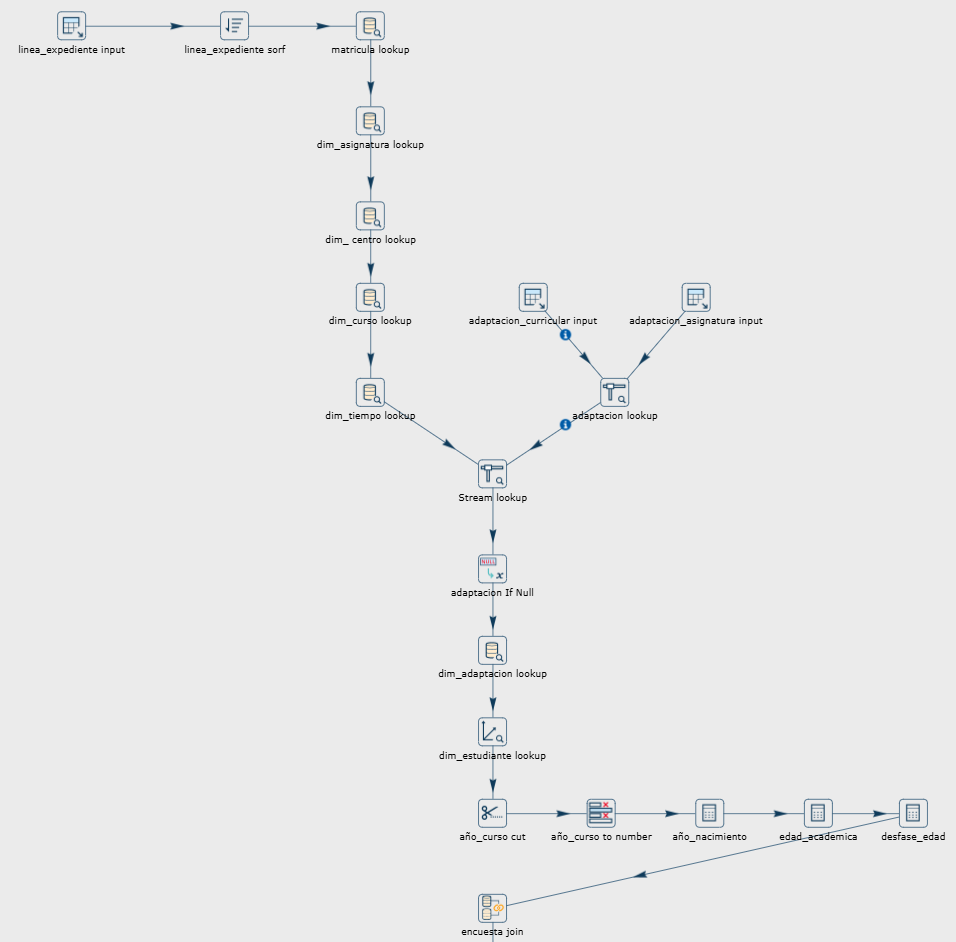
\includegraphics[width=1\textwidth]{imaxes/fact_calificaciones_p1.png}
    \caption{Flujo del pipeline \textit{fact\_calificaciones.hpl} (Parte 1).}
    \label{fig:fact_calificaciones_p1}
\end{figure}

\begin{figure}[htbp]
    \centering
    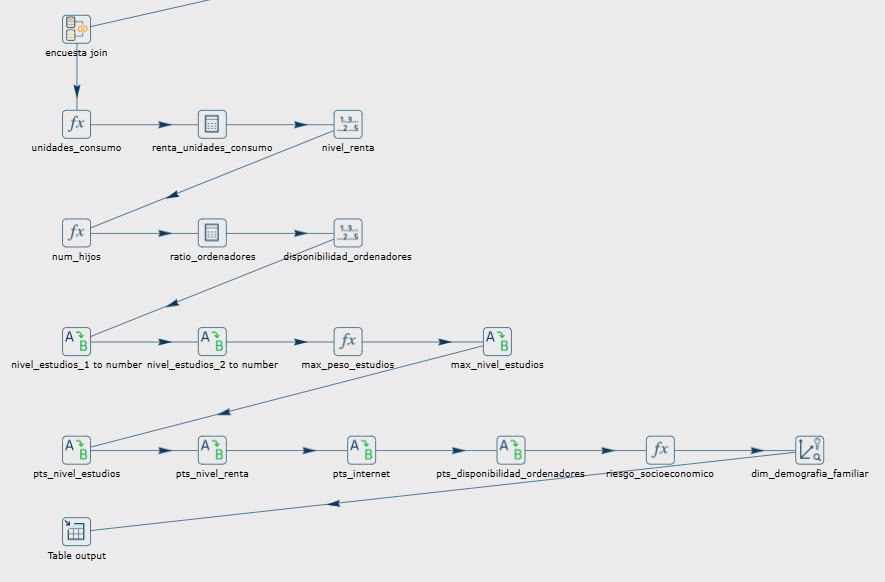
\includegraphics[width=1\textwidth]{imaxes/fact_calificaciones_p2.png}
    \caption{Flujo del pipeline \textit{fact\_calificaciones.hpl} (Parte 2).}
    \label{fig:fact_calificaciones_p2}
\end{figure}

\subsection{Tabla de Hechos de rendimiento por Evaluación}

El último pipeline del ecosistema ETL actúa como el motor predictivo del proyecto, consolidando las calificaciones para calcular el riesgo final de abandono escolar. Para poder nutrir gráficos de tendencia dinámicos y, simultáneamente, penalizar el riesgo si el alumno arrastra fracasos previos, el pipeline abandona la clásica consolidación estática anual y adopta una arquitectura de "Suma Acumulada" manteniendo el grano de la tabla a nivel de Evaluación (\textit{id\_estudiante} $\times$ \textit{id\_tiempo}).

\begin{enumerate}
    \item \textbf{Ingesta y Tipificación Analítica (\textit{Table Input}, \textit{DBLookup} y \textit{Formula}):} El flujo ingiere \textit{dwh.fact\_calificaciones} y cruza mediante \textit{DBLookup} con todas las dimensiones clave (\textit{dim\_tiempo}, \textit{dim\_curso}, \textit{dim\_demografia\_familiar}, \textit{dim\_adaptacion}). Tras esto, un nodo \textit{Formula} bautizado como ``flags analíticos'' perfila las casuísticas de cada nota. Es aquí donde se detecta de forma temprana si el registro pertenece al ciclo crítico de 1º y 2º de Primaria (\textit{is\_prim\_1\_2}), y se despliegan vectores binarios para segmentar si un suspenso es de evaluación final o parcial, y si pertenece a dicho ciclo crítico o al resto.
    \item \textbf{Rastreo Histórico Acumulado (Flujo Principal):} Tras una ordenación cronológica estricta (\textit{id\_estudiante} $\times$ \textit{curso\_academico} $\times$ \textit{orden\_evaluacion}), un nodo \textit{Group By} agrupa por estudiante activando la directiva \textit{"Include all rows"}. Implementando funciones \textit{Cumulative sum} sobre los vectores previamente generados, el sistema emula una \textit{Window Function}. Esto arrastra en el registro actual todo el bagaje histórico de suspensos segmentados (parciales/finales y primaria/resto).
    \item \textbf{Motor Detección de Repetidores (Sub-rama Paralela):} El flujo se bifurca hacia una rama auxiliar especializada en trazar las repeticiones. Puesto que los parciales duplican los cursos, un nodo \textit{Group By} colapsa la granularidad a un solo registro por año. Posteriormente, un nodo \textit{Analytic Query} (LAG 1) lee el \textit{curso\_anterior} del alumno. Un nodo \textit{Formula} detecta matemáticamente la repetición y separa mediante \textit{flags} si esta se produce en 1º/2º de Primaria o en cursos superiores. Finalmente, un segundo \textit{Group By} con sumatoria acumulativa calcula el cómputo histórico de repeticiones del alumno (\textit{num\_repetir\_1\_2\_pri} y \textit{num\_repetir\_resto}).
    \item \textbf{Fusión y Reencuentro (\textit{StreamLookup}):} Tras calcular la historia de repeticiones de la sub-rama, se hace un cruce (Left Join en memoria) mediante el nodo \textit{StreamLookup}. Este vuelve a inyectar al flujo principal transaccional toda la mochila de repeticiones basándose en la clave \textit{id\_estudiante} $\times$ \textit{curso\_academico}.
    \item \textbf{Ecuación Maestra de Riesgo (\textit{Formula}):} Un potente nodo de fórmulas se encarga de convertir todas las acumulaciones en puntuaciones predictivas (Scoring). El \textbf{Riesgo Académico} se calcula ponderando de manera asimétrica los factores: suspensos finales en 1º/2º Primaria (20 pts), suspensos parciales (10 pts) y penalizando drásticamente la repetición en este ciclo temprano (40 pts), frente a las métricas del resto de cursos que tienen un peso menor. A la par, evalúa el riesgo base familiar creando una puntuación escalonada para el \textbf{Riesgo Socioeconómico} (10 pts si supera el umbral severo, 5 si es riesgo moderado).
    \item \textbf{Cálculo del Indicador de Abandono (\textit{Calculator}):} Como culminación, un nodo sumatorio simple (\texttt{ADD3}) consolida matemáticamente el \textit{riesgo\_academico}, el \textit{riesgo\_adaptacion} y los puntos socioeconómicos. Esto arroja el indicador definitivo \textit{riesgo\_abandono}, que finalmente es almacenado en la tabla \textit{dwh.fact\_rendimiento\_anual} a través de un nodo \textit{Table Output}.
\end{enumerate}

\begin{figure}[htbp]
    \centering
    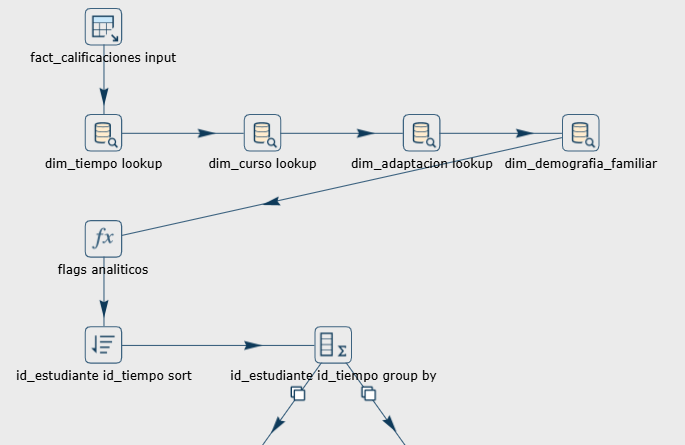
\includegraphics[width=1\textwidth]{imaxes/fact_rendimiento_anual_p1.png}
    \caption{Flujo del pipeline \textit{fact\_rendimiento\_anual.hpl} (Parte 1).}
    \label{fig:fact_rendimiento_anual_p1}
\end{figure}

\begin{figure}[htbp]
    \centering
    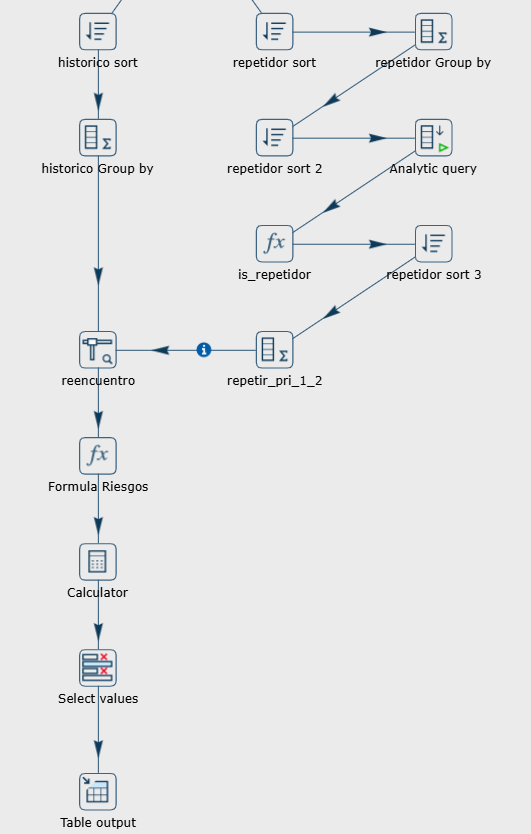
\includegraphics[width=1\textwidth]{imaxes/fact_rendimiento_anual_p2.png}
    \caption{Flujo del pipeline \textit{fact\_rendimiento\_anual.hpl} (Parte 2).}
    \label{fig:fact_rendimiento_anual_p2}
\end{figure}

\section{Orquestación y Workflows}

Todos estos pipelines independientes (\textit{.hpl}) son llamados y secuenciados por flujos de trabajo o \textit{Workflows} (\textit{.hwf}). Mientras que los pipelines manejan registros fila a fila, los workflows manejan la lógica de control a nivel de proceso.

La orquestación del proyecto sigue una arquitectura jerárquica encabezada por el flujo principal \textit{main.hwf} (ver Figura \ref{fig:main_workflow}), el cual delega la carga en dos sub-workflows de especialidad:

\begin{enumerate}
    \item \textbf{\textit{dimensions.hwf}:} Este flujo se encarga de la extracción inicial y la carga de dimensiones (ver Figura \ref{fig:dimensions_workflow}). Su ejecución comienza disparando el pipeline de extraccion a \textit{Staging}. Una vez los datos están en bruto en el esquema \textit{raw}, el workflow lanza en \textbf{paralelo} la carga de todas las dimensiones (\textit{dim\_tiempo}, \textit{dim\_curso}, \textit{dim\_estudiante}, etc.) para maximizar el rendimiento. Es crítico que todas finalicen con éxito para garantizar la integridad referencial.
    \item \textbf{\textit{facts.hwf}:} Tras asegurar las dimensiones, \textit{main.hwf} dispara este segundo sub-workflow (ver Figura \ref{fig:facts_workflow}). A diferencia del anterior, se ejecuta de manera estrictamente secuencial: primero el flujo de calificaciones (para asegurar la granularidad atómica) y, solo si este finaliza correctamente, el pipeline de rendimiento por evaluación (encargado de las agregaciones finales).
\end{enumerate}

\subsection{Manejo de Errores Multinivel (\textit{Error Handling})}

La robustez del sistema recae en un diseño de gestión de excepciones presente en todas las capas. Tanto el \textit{main.hwf} como los sub-workflows (\textit{dimensions.hwf} y \textit{facts.hwf}) implementan bloques de captura de errores. 

Si cualquier pipeline de transformación individual reporta un fallo (por ejemplo, una clave foránea huérfana), el sub-workflow correspondiente detiene su rama de ejecución y se desvía hacia una acción \textit{Write to log}. Allí registra la incidencia ("Uno de los pipelines de dimensión ha fallado") y lanza un \textit{Abort workflow}. Este fallo se propaga jerárquicamente hacia arriba hasta el \textit{main.hwf}, que también registra su propio error crítico y aborta la orquestación global. Esta topología previene cualquier corrupción o carga parcial en el Data Warehouse.

\begin{figure}[htbp]
    \centering
    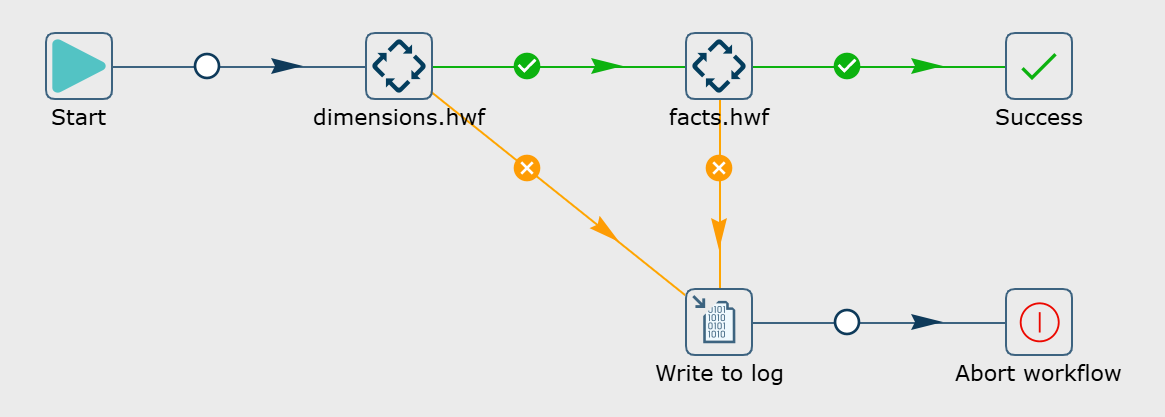
\includegraphics[width=1\textwidth]{imaxes/main_workflow.png}
    \caption{Workflow principal (\textit{main.hwf}) y su delegación jerárquica en sub-flujos.}
    \label{fig:main_workflow}
\end{figure}

\begin{figure}[htbp]
    \centering
    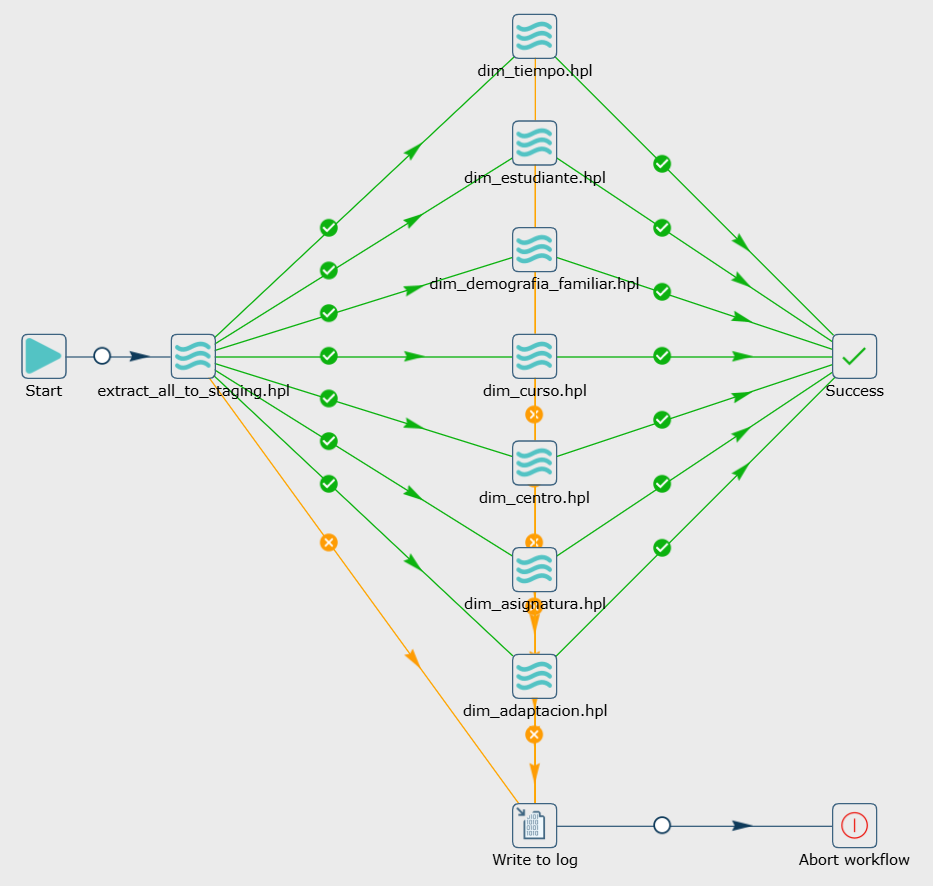
\includegraphics[width=1\textwidth]{imaxes/dimensions_workflow.png}
    \caption{Sub-flujo de dimensiones (\textit{dimensions.hwf}) ejecutado en paralelo.}
    \label{fig:dimensions_workflow}
\end{figure}

\begin{figure}[htbp]
    \centering
    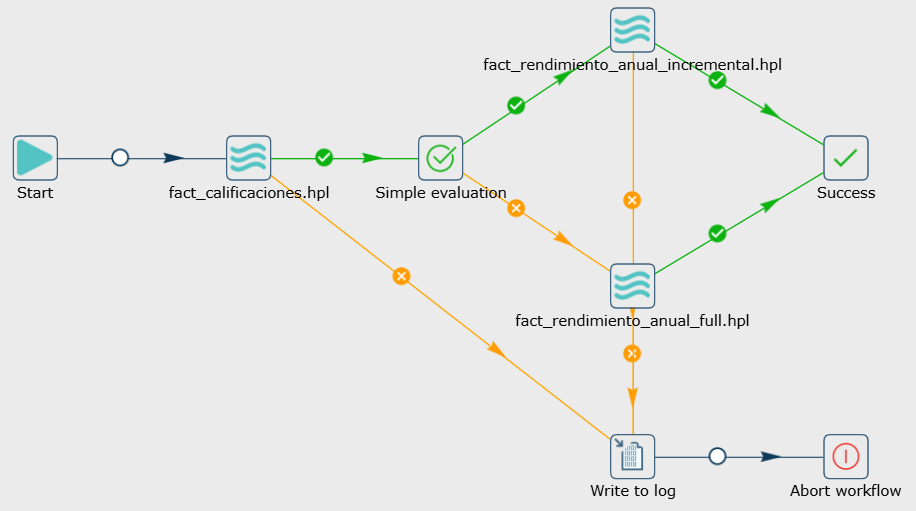
\includegraphics[width=1\textwidth]{imaxes/facts_workflow.png}
    \caption{Sub-flujo de hechos (\textit{facts.hwf}) ejecutado de forma secuencial.}
    \label{fig:facts_workflow}
\end{figure}
